%%% LaTeX Template: Article/Thesis/etc. with colored headings and special fonts
%%%
%%% Source: http://www.howtotex.com/
%%% Feel free to distribute this template, but please keep to referal to http://www.howtotex.com/ here.
%%% February 2011
%%%
%%% Modified January 2018 by CDM

%%%  Preamble
\documentclass[11pt,letterpaper]{article}
\usepackage[margin=1.0in]{geometry}
\usepackage[T1]{fontenc}
\usepackage[bitstream-charter]{mathdesign}
\usepackage[latin1]{inputenc}					
\usepackage{amsmath}						
\usepackage{xcolor}
\usepackage{cite}
\usepackage{hyphenat}
\usepackage{graphicx}
\usepackage{float}
\usepackage{subfigure}
\usepackage{sectsty}
\usepackage[compact]{titlesec} 
\usepackage[tablegrid]{vhistory}
\allsectionsfont{\color{accentcolor}\scshape\selectfont}

%%% Definitions
\definecolor{accentcolor}{rgb}{0.0,0.0,0.5} 
\newcommand{\teamname}{Team Name}
\newcommand{\productname}{Product Name}
\newcommand{\coursename}{CSE 4316: Senior Design I}
\newcommand{\semester}{Spring 2018}
\newcommand{\docname}{System Requirements Specification}
\newcommand{\department}{Department of Computer Science \& Engineering}
\newcommand{\university}{The University of Texas at Arlington}
\newcommand{\authors}{Alan Turing \\ Grace Hopper \\ John Von Neumann \\ Ada Lovelace \\ Charles Babbage}

%%% Headers and footers
\usepackage{fancyhdr}
	\pagestyle{fancy}						% Enabling the custom headers/footers
\usepackage{lastpage}	
	% Header (empty)
	\lhead{}
	\chead{}
	\rhead{}
	% Footer
	\lfoot{\footnotesize \teamname \ - \semester}
	\cfoot{}
	\rfoot{\footnotesize page \thepage\ of \pageref{LastPage}}	% "Page 1 of 2"
	\renewcommand{\headrulewidth}{0.0pt}
	\renewcommand{\footrulewidth}{0.4pt}

%%% Change the abstract environment
\usepackage[runin]{abstract}			% runin option for a run-in title
%\setlength\absleftindent{30pt}			% left margin
%\setlength\absrightindent{30pt}		% right margin
\abslabeldelim{\quad}	
\setlength{\abstitleskip}{-10pt}
\renewcommand{\abstractname}{}
\renewcommand{\abstracttextfont}{\color{accentcolor} \small \slshape}	% slanted text

%%% Start of the document
\begin{document}

%%% Cover sheet
{\centering \huge \color{accentcolor} \sc \textbf{\department \\ \university} \par}
\vspace{1 in}
{\centering \huge \color{accentcolor} \sc \textbf{\docname \\ \coursename \\ \semester} \par}
\vspace{0.5 in}
\begin{figure}[h!]
	\centering
   	
\includegraphics[width=0.60\textwidth]{images/test_image}
\end{figure}
\vspace{0.5 in}
{\centering \huge \color{accentcolor} \sc \textbf{\teamname \\ \productname} \par}
\vspace{0.5 in}
{\centering \large \sc \textbf{\authors} \par}
\newpage


%\vspace{1 in}
%\centerline{January 13th, 2012}
%\newpage

%%% Revision History
\begin{versionhistory}
  	\vhEntry{0.1}{10.01.2015}{GH}{document creation}
  	\vhEntry{0.2}{10.05.2015}{AT|GH}{complete draft}
  	\vhEntry{0.3}{10.12.2015}{AT|GH}{release candidate 1}
  	\vhEntry{1.0}{10.20.2015}{AT|GH|CB}{official release}
  	\vhEntry{1.1}{10.31.2015}{AL}{added customer change requests}
\end{versionhistory}
\newpage

%%% Table of contents
\setcounter{tocdepth}{2}
\tableofcontents
\newpage

%%% List of figures and tables (optional)
\listoffigures
%\listoftables
\newpage

\section{Product Concept}
This section provides a high-level statement of your product concept - what it is intended to do and how it is intended to be used. Include in this header paragraph, a brief synopsis of what is described here. For example, this header paragraph might say something like: "This section describes the purpose, use and intended user audience for the X product. X is a system that performs Y. Users of X will be able to Z..."

\subsection{Purpose and Use}
This is where you describe in a brief, yet clear and concise, manner what your product should do and how you expect it should be used.

\subsection{Intended Audience}
This is where you describe the intended audience(s) of your product. If this product were to be made available publicly or commercially, who would purchase or use it? Is the product designed for a particular customer, or an overall class of customers? Is it intended for general use, or is it a specific component of a more complex system?

\begin{figure}[h!]
	\centering
   	
\includegraphics[width=0.60\textwidth]{images/test_image}
    \caption{X conceptual drawing}
\end{figure}

\newpage
\section{Product Description}
The overview of Bluetooth Hydrometer is provided in this section. Arduino Nano 33 BLE is a microcontroller used for Bluetooth Hydrometer. Nano 33 is a small and low powered Bluetooth enabled device with a built in 9-axis gyroscope. Nano operates at 3.3 V, it has 14 digital inputs, 8 analog inputs and 6 power modulations (PWM) and a clock speed of 64 MHz. Temperature sensor used operates at 3.3V with temperature range of $-$40 to 125$^\circ$C having an accuracy of  $\pm$1.5$^\circ$C.

\begin{figure}[h!]
	\centering
   	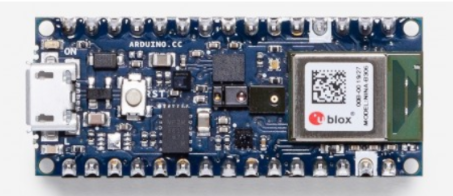
\includegraphics[width=0.60\textwidth]{images/arduino_nano_33}
    \caption{Arduino Nano 33}
\end{figure}
\begin{figure}[h!]
	\centering
   	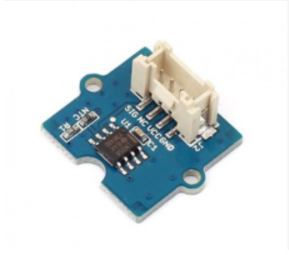
\includegraphics[width=0.60\textwidth]{images/temperature_sensor}
    \caption{Temperature Sensor}
\end{figure}

\subsection{Features \& Functions}
What the product does and does not do. Specify in words what it looks like, referring to a conceptual diagram/graphic (Figure X).  Define the principle parts/components of the product. Specify the elements in the diagram/graphic that are part(s) of this product as well as any associated external elements (e.g., the Internet, an external web server, a GPS satellite, etc.)

\subsection{External Inputs \& Outputs}
External input is temperature and specific gravity data from temperature sensor and built in gyroscope sensor respectively. Arduino nano outputs those data to smartphones via Bluetooth and a website.

\subsection{Product Interfaces}
Bluetooth module plays an important role to interface nano. Datas are constantly uploaded via Bluetooth to a smartphone or a website. Nano can be interfaced  to send data only after a certain time interval, since temperature and SG don't change every second or minute. Software can handle and analyze those datas within an app or a website to provide visual interface to users.

\newpage
\section{Customer Requirements}
Include a header paragraph specific to your product here. Customer requirements are those required features and functions specified for and by the intended audience for this product. This section establishes, clearly and concisely, the "look and feel" of the product, what each potential end-user should expect the product do and/or not do. Each requirement specified in this section is associated with a specific customer need that will be satisfied. In general Customer Requirements are the directly observable features and functions of the product that will be encountered by its users. Requirements specified in this section are created with, and must not be changed without, specific agreement of the intended customer/user/sponsor.

\subsection{Requirement Name}
\subsubsection{Description}
A detailed description of the feature/function that satisfies the requirement. For example: \textit{The box will be slate blue. This specific color is required in order to ensure that the box matches other similar boxes in the Box Systems Premium line of products. Slate blue is specified as \#007FFF, using six-digit hexadecimal color specification.} It is acceptable and advisable to include drawings/graphics in the description if it aids understanding of the requirement.
\subsubsection{Source}
The source of the requirement (e.g. customer, sponsor, specified team member (by name), federal regulation, local laws, CSE Senior Design project specifications, etc.)
\subsubsection{Constraints}
A detailed description of constraints on satisfying the requirement (e.g. one such constraint might be: \textit{The specified color must be commercially available in paint capable of adhering to the material of which the box is manufactured. (See customer requirement 3.x for production material specification.)}
\subsubsection{Standards}
A detailed description of any specific standards that apply to this requirement (e.g. \textit{NSTM standard xx.xxx.x. color specifications \cite{Rubin2012}}.)
\subsubsection{Priority}
The priority of this requirement relative to other specified requirements. Use the following priorities:
\begin{itemize}
\item Critical (must have or product is a failure)
\item High (very important to customer acceptance, desirability)
\item Moderate (should have for proper product functionality);
\item Low (nice to have, will include if time/resource permits)
\item Future (not feasible in this version of the product, but should be considered for a future release).
\end{itemize}

\subsection{Requirement Name}
\subsubsection{Description}
Detailed requirement description...
\subsubsection{Source}
Source
\subsubsection{Constraints}
Detailed description of applicable constraints...
\subsubsection{Standards}
List of applicable standards
\subsubsection{Priority}
Priority

\newpage
\section{Packaging Requirements}
Include a header paragraph here. Packaging requirements are those requirements that identify how the delivered product will be packaged for delivery to the end-user; or how it will "look" when finished and delivered. For example, you might specify that the software required for operation will be pre-loaded on the hard drive, delivered on CD/DVD, or available via download. Software might be customer installable, or not, etc. Hardware components could be all in a single package, provided as a "bag of parts" to be assembled/installed by the user, painted a certain color, logos affixed, etc. Care should be taken not to duplicate requirements found in other sections of this document.

\subsection{Requirement Name}
\subsubsection{Description}
Detailed requirement description...
\subsubsection{Source}
Source
\subsubsection{Constraints}
Detailed description of applicable constraints...
\subsubsection{Standards}
List of applicable standards
\subsubsection{Priority}
Priority
\newpage
\section{Performance Requirements}
This section outlines performance-related requirements. The bluetooth hydrometer relies heavily on communication between the user's mobile application control, reliability of the battery module, and optimization of communication between the application and module.

\subsection{Battery Usage}
\subsubsection{Description}
The battery must be able to be kept on for a total of 2 months minimum. When turned off and the bluetooth module is off, no battery power must be consumed.
\subsubsection{Source}
This is a bare necessity requirement for operation, as the hydrometer must be able to stay on for a long enough total time to last for the duration of short checks along the period of a brew.
\subsubsection{Constraints}
The 9V battery module is a set 1,200mAh capacity, so the load must be small enough to sustain power for the required length of time.
\subsubsection{Standards}
Not applicable.
\subsubsection{Priority}
This requirement is important for having the use load remain low, but not critical as the hydrometer is a device that does not require much power for basic operation and will already last a long enough time for several checks.
\subsection{Speed Of Setup}
\subsubsection{Description}
Turning the module on will take no longer than 60 seconds to set up with the mobile application. By pressing a button in the application for turning on the hydrometer, a signal should be sent to the web server to indicate power and data to start to be read in. This is excluding the time to assemble the hydrometer and place it in the brew container.
\subsubsection{Source}
This is a group requirement for the end user. Having the hydrometer respond to the control application in a reasonable amount of time is essential to having the user experience be quick. 
\subsubsection{Constraints}
The 9V battery module is a set 1,200mAh capacity, so the load must be small enough to sustain power for the required length of time.
\subsubsection{Standards}
Not applicable.
\subsubsection{Priority}
This is critical to using the hydrometer, as taking longer than 60 seconds to just turn on the device would become a burden to the user for a time-sensitive project like brewing.
\subsection{Accuracy Of Results}
\subsubsection{Description}
Reading the specific gravity will return a calculated sugar level result to the user that is correct with less than a 5\% error. Multiple readings will be continuously sent to the server, where all the data will be processed to return a specific gravity answer to the user through the mobile application.
\subsubsection{Source}
This is a project requirement, as the whole point of the device is to give a reading of one measurement, the sugar level.
\subsubsection{Constraints}
To measure any tilt, a baseline angle of tilt must be noted as a neutral starting position. The code will include an initial reading of tilt at the start of the brew.
\subsubsection{Standards}
Not applicable.
\subsubsection{Priority}
This is the highest priority requirement of the project, as incorrect readings will hinder the resultant brew and may cause the user to take too long or too short of a time to end the brew.
\newpage
\section{Safety Requirements}
This section details the safety requirements to the bluetooth hydrometer use. The risk factors of the hydrometer being a low-voltage electrical device is that it may pose a slight electrocution risk to the end-user, and a short-circuit may damage the electronic components of the hydrometer including the main Arduino board.

\subsection{Requirement Name}
\subsubsection{Description}
As the bluetooth hydrometer is going to be a device that is placed in liquid for use, it is important to ensure that the outer capsule is kept closed and sealed to the entirety of the time it is used. The user must ensure that he/she is grounded before working with the hydrometer.
\subsubsection{Source}
This is a basic project safety requirement to make sure that the user does not get electric shocked and that the device does not become short circuited.
\subsubsection{Constraints}
The user will be handling the Arduino board directly as it has no other protective covering when outside of the outer capsule.
\subsubsection{Standards}
Not applicable.
\subsubsection{Priority}
This is of critical importance for device use.
\newpage
\section{Maintenance \& Support Requirements}
There should be a portal for the customers to leave suggestions and feedback and report problems. There also need to be an RMA, so customers can return the product if it's defective or they simply don't want it for a refund.

\subsection{Users shall be able to get support on any issues}
\subsubsection{Description}
The must be a website with a portal where customers can create a profile if they wish. Customers aren't require to have a profile if they preferred not to have a profile. Customer can also either leave a suggestion or a feedback for the app through the website or through the Google Play store. The portal on the website should have an FAQ section for questions that customers generally have about the app and the hydrometer.

There should be a community section where customers can discuss among themselves, the producers of the product, and the developers of the app about any issues, concerns, or questions. The customers should also be able to report any issues directly to us through the website and we should be able to address it with them if they wish. Customers should also be able to contact customer support through email or a hot line in case they have any issues, concerns, or questions.

We must be able to create an RMA (Return Merchandise Authorization) with any customers that have issues with their product. The RMA allows the customer to send the product back if it's having issues so we can repair it and send it back to them or we can send them a another one. Each customer has a full one-year warranty coverage on the product. The warranty policy will cover the cost of repairing or replacing the product if the product fails within the one-year period due to manufacturer defect.

Customers also have the option to return the product for a full refund within 30 days if whether the product failed or if the product failed to perform what the customers expected or even if the customers simply doesn't want the product.
\subsubsection{Source}
The source is from my own understanding of customer and technical support.
\subsubsection{Constraints}
The warranty will not cover repair or replacement cost of products if it becomes defective one-year after it had been shipped. The warranty will not cover damages that aren't caused by manufacturer defect.

If a customer wanted to return a product for a full refund just because they don't want it and that the customer couldn't provide us any proof of manufacturer defect or why the product doesn't perform as the customer expected. Then the customer will be required to pay a restocking fee for return the product.
\subsubsection{Standards}
This product is governed by Consumer Protection.
\subsubsection{Priority}
This requirement is somewhat important. It is not something we shall worry to much about, but it's important when the products failed to perform what the customers expected.
\newpage
\section{Other Requirements}
This section details additional requirements that vary in categorization.

\subsection{Operating System Compatibility}
\subsubsection{Description}
The bluetooth hydrometer software will be developed on Linux, Windows 10, and MacOS by different group members. The project will be written with the end user using Linux in mind. Android is required to use the mobile control application.
\subsubsection{Source}
Each member has a different OS he/she prefers to work on, but Linux will be used for ease of collaboration. iOS is a less modular and less forgiving OS to develop for.
\subsubsection{Constraints}
As each operating system may have slight variations in how programs are run or deals with external hardware, there may need additional collaboration and communication among team members to continue development.
\subsubsection{Standards}
Not applicable.
\subsubsection{Priority}
As it isn't known yet if the device, application, and server would work the same in other operating systems with no additional development needed, this requirement is of average or below average importance.
\subsection{Product Shell}
\subsubsection{Description}
The Arduino board and components will be encased in a capsule to have it float in a brew liquid. Other than the shell, there will be no other covering or protection of the device.
\subsubsection{Source}
This is the simplest method for allowing the device to float without superfluous features that may interfere with tilt readings.
\subsubsection{Constraints}
The capsule must hold the device without having the Arduino move inside. It must also seal completely tight so that no liquid reaches the Arduino or components.
\subsubsection{Standards}
Not applicable.
\subsubsection{Priority}
Critical to having the device in brew at all.
\subsection{Languages \& Additional Software}
\subsubsection{Description}
The bluetooth hydrometer software will be developed on Linux, Windows 10, and MacOS by different group members. Primarily, the project will be written in C, with possible additional code written in SQL should a database be required with the web server. Github will be used for remote sharing.
\subsubsection{Source}
Android development and Arduino development are both in C.
\subsubsection{Constraints}
Each team member must be able to adequately write, read, and understand C and each aspect of the project, as all software components work in tandem for full functionality. 
\subsubsection{Standards}
Not applicable.
\subsubsection{Priority}
As conversion to different languages via modules is possible but comes with potential for multiple issues and bugs, this requirement is of above average importance.
\newpage
\section{Future Items}
In this last section, you will reiterate all requirements that are listed as priority 5. This is repetitive, but necessary as a concise statement of features/functions that were considered/discussed and documented herein, but will NOT be addressed in the prototype version of the product due to constraints of budget, time, skills, technology, feasibility analysis, etc. Use the following format for this section.

\subsection{Requirement Name}
\subsubsection{Description}
Detailed requirement description...
\subsubsection{Source}
Source
\subsubsection{Constraints}
Detailed description of applicable constraints...
\subsubsection{Standards}
List of applicable standards
\subsubsection{Priority}
Priority
\newpage

%%% References
\bibliographystyle{plain}
\bibliographystyle{reference/IEEEtran_custom}
\bibliography{reference/refs}{}

\end{document}